\section{実験方法}
カーレースAIのサンプルを改善するために,車の操作用のスクリプトからトラックやチェックポイントまで全てを変更する必要があるので,スクラッチから新しい車エージェントや環境を作成することがより効率的だと判断した.以下では,スクラッチからの環境構築プロセスについて説明する.
この章では,カリキュラム学習のアプローチを用いて学習を進めた.カリキュラム学習は,学習期間の短縮やモデルの精度向上のために,段階的に難易度を上げる手法である.

\subsection{道路の環境構築}
Unityのアセットストアから無料のシティ(City)モデルやスポーツカー(Sports Car)モデルをダウンロードした.
新しい道路のシンプルなレイアウトを作成し,手に入れたモデルをエディタ内に配置した.モデルを配置する際,学習時に問題が生じないようにモデルのサイズや位置を正確に設定した.新しい道路の壁には凸凹があったため,道路上に見えない直方体を作成し,壁を滑らかにした.滑らかにした状態を以下の図4に示す.
\begin{figure}[H]
    \centering
    \includegraphics[width=0.8\textwidth]{figures/invisible-wall.eps} % ここで図のファイル名とサイズを指定します
    \caption{滑らかにした道路の壁} % 図のキャプション
    \label{fig:invisible-wall} % 図への参照用ラベル
\end{figure}

\subsubsection{チェックポイントの配置}
新しい道路完成後,トラック上に56個の見えないチェックポイントを配置した.どのチェックポイントを通過したかを追跡するために,チェックポイント管理システムのスクリプトを作成し,それを各チェックポイントに付けた.このシステムでは,車が特定のチェックポイントを通過すると,そのチェックポイントのタグをシステムに更新する.全てのチェックポイントを通過した後,チェックポイントのタグはリセットされる.シチモデルと配置したチェックポイントの様子を以下の図5に示す.
\begin{figure}[H]
    \centering
    \includegraphics[width=0.8\textwidth]{figures/checkpoints.eps} % ここで図のファイル名とサイズを指定します
    \caption{配置されたチェックポイント} % 図のキャプション
    \label{fig:checkpoints} % 図への参照用ラベル
\end{figure}


\subsection{車エージェントの作成}
アセットストアからダウンロードしたモデルに適切なボディとタイヤのコライダーを設定し,モデルに合わせた.また,車モデルにリジッドボディ(Rigidbody)を付けて重力を受けるように設定した.リジッドボディとは,ゲームオブジェクトを物理特性によって制御することができるようにするコンポネントである.作成した車エージェントのモデルを以下の図6に示す.
\begin{figure}[H]
    \centering
    \includegraphics[width=0.8\textwidth]{figures/car1.eps} % ここで図のファイル名とサイズを指定します
    \caption{車エージェントのモデル} % 図のキャプション
    \label{fig:car-model} % 図への参照用ラベル
\end{figure}


\subsubsection{エージェントの Raycast 3D センサーの設定}
車が周囲の環境を正確に認識できるように,2種類の Raycast 3D センサーを設定した.1つ目のセンサーは車の前半部分の約180度にわたり15本のセンサーで,近くの壁やチェックポイントを識別する.作成した1つ目のセンサーとその設定を図7,図8に示す.\\
\begin{figure}[H]
    \centering
    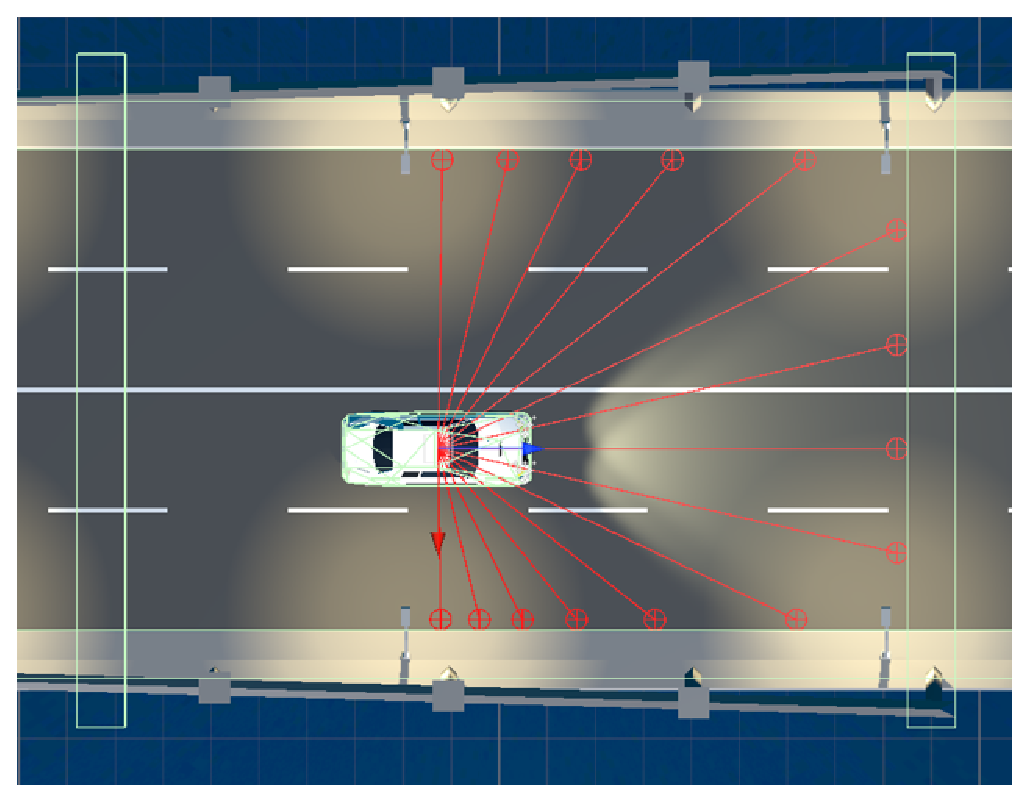
\includegraphics[width=0.8\textwidth]{figures/FirstRaycast.eps} % ここで図のファイル名とサイズを指定します
    \caption{1つ目のRayCastセンサー} % 図のキャプション
    \label{fig:first-raycast} % 図への参照用ラベル
\end{figure}

\begin{figure}[H]
    \centering
    \includegraphics[width=0.8\textwidth]{figures/FirstRaycastSettings.eps} % ここで図のファイル名とサイズを指定します
    \caption{1つ目のRayCastセンサーの設定} % 図のキャプション
    \label{fig:first-raycast-settings} % 図への参照用ラベル
\end{figure}

2つ目のセンサーは車の前方約90度にわたり13本のセンサーで,遠くの壁や障害物を識別する.これにより,車がスムーズに道路を進めるように各センサーがそれぞれの役割を果たす.作成した2つ目のセンサーとその設定を図9,図10に示す.
\begin{figure}[H]
    \centering
    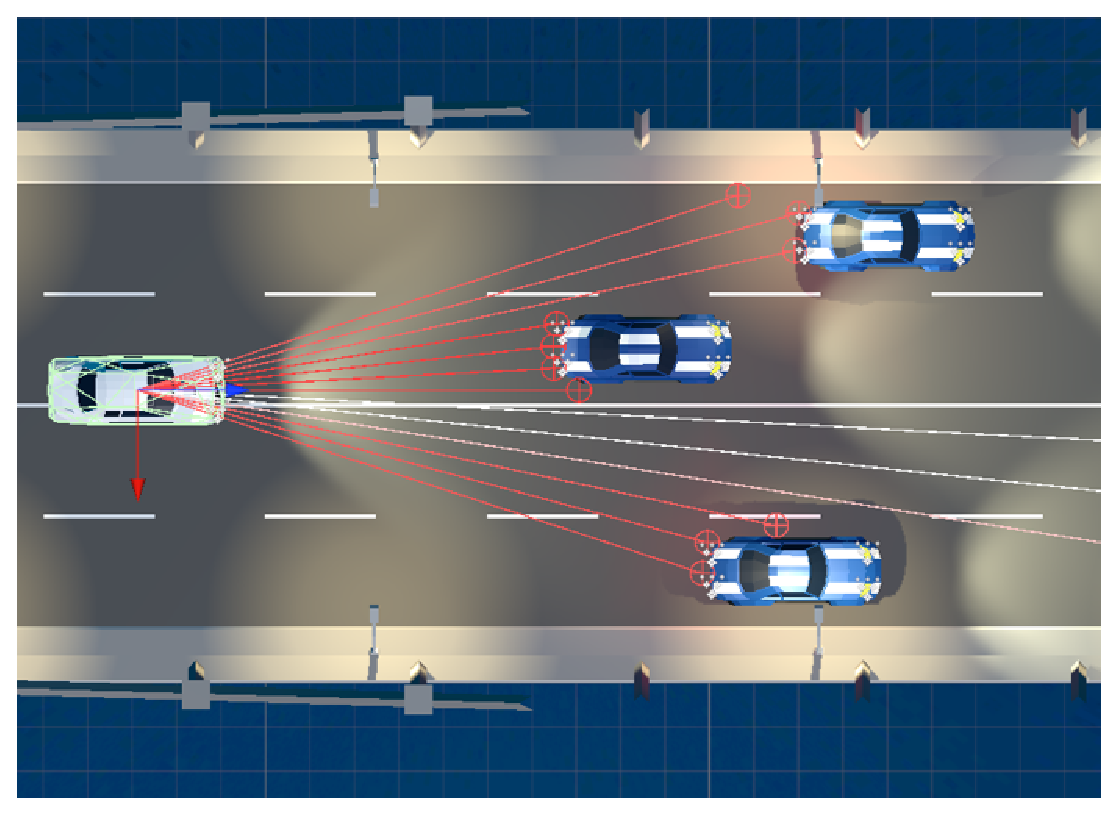
\includegraphics[width=0.8\textwidth]{figures/SecondRaycast.eps} % ここで図のファイル名とサイズを指定します
    \caption{2つ目のRayCastセンサー} % 図のキャプション
    \label{fig:second-raycast} % 図への参照用ラベル
\end{figure}

\begin{figure}[H]
    \centering
    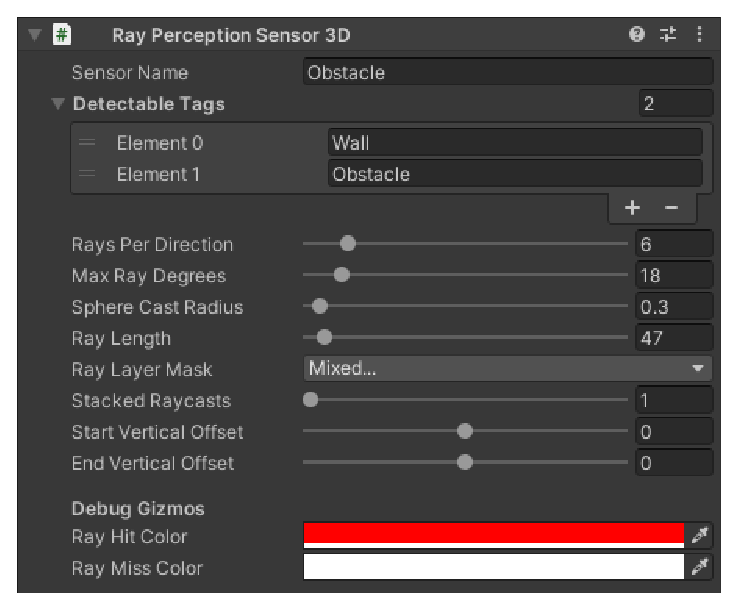
\includegraphics[width=0.8\textwidth]{figures/SecondRaycastSettings.eps} % ここで図のファイル名とサイズを指定します
    \caption{2つ目のRayCastセンサーの設定} % 図のキャプション
    \label{fig:second-raycast-settings} % 図への参照用ラベル
\end{figure}

\subsubsection{操作用のスクリプト}
エージェントに与えられた基本操作はアクセル,ブレーキ,および左右のステアリングである.ブレーキに関しては,通常のレーシングゲームでは完全に停止すると後退し始めるが,本研究ではハンドブレーキのように設定し,速度がゼロになると車は動かなくなるようにした.これは,学習中に車が不必要に後退することを防ぐためである.

\subsubsection{学習用のエージェントスクリプトの詳細}
学習プロセスを最適化するために,エージェントスクリプトでは様々なシナリオでの報酬とペナルティが設定されている.これにより,車エージェントは効率的に適切な行動を学習し,不適切な行動を避けることができる.
\begin{enumerate}
  \item OnEpisodeBegin()では,各エピソード開始時に車と障害物の位置と速度をリセットし,前のエピソードからの影響を排除する.これにより,エージェントが新しいエピソードでスムーズな状態から始めることができる.
  \item CollectObservations()では,エージェントは自信の位置や速度および次のチェックポイントの位置情報を収集する.これらの情報を基にエージェントは次の行動を決定する.
  \item OnActionReceived()では,エージェントの行動に基づいて報酬やペナルティが与えられる.これにより,エージェントは有益な行動を強化し,不利益な行動を避けるように学習する.
\end{enumerate}

\subsection{報酬システムの詳細}
\subsubsection{報酬(Reward)}
\begin{enumerate}
  \item \textbf{速度維持報酬:}
エージェントが一定の速度基準を超えると,小さな報酬(+0.0001f)が与えられる.これは車に速い走行を促すためである.
  \item \textbf{チェックポイント通過報酬:}
車が道路上に配置された見えないチェックポイントを通過するたびに,より大きな報酬(+0.5f)が与えられる.
\end{enumerate}

\begin{figure}[H]
    \centering
    \includegraphics[height=0.4\textheight]{figures/CheckpointReward.eps} % ここで図のファイル名とサイズを指定します
    \caption{チェックポイントを通過する度の報酬} % 図のキャプション
    \label{fig:checkpoint-reward} % 図への参照用ラベル
\end{figure}

\subsubsection{罰(Penalty)}
\begin{enumerate}
  \item \textbf{一定のペナルティ:}車には1ステップごとに(1ステップ=20ms)小さなペナルティ(-0.0001f)が与えられる.これは車が停止し続けるとペナルティが加算されるため,車が動き続けるように促すためである.
  \item \textbf{原則ペナルティ:}車が減速して速度がゼロになった場合は,車にペナルティ(-0.5f)が与えられ,車の状態がリセットされる.
  \item \textbf{学習難易度に応じて衝突したペナルティの調整:}壁や障害物に衝突した場合,学習の初期モデルでは小さめなペナルティを設定し,難易度が上がるにつれてペナルティ(-0.5fから-2.0fまで)増加させる.車が障害物に衝突した様子を図12に示す.
\end{enumerate}

\begin{figure}[H]
    \centering
    \includegraphics[height=0.4\textheight]{figures/CarCollision.eps} % ここで図のファイル名とサイズを指定します
    \caption{衝突した様子} % 図のキャプション
    \label{fig:car-collision} % 図への参照用ラベル
\end{figure}

\subsection{障害物の作成と操作スクリプト}
障害物(他車)はルールベースのAIによって制御され,指定された車線(レーン)を走行する.このAIは,レーン内の特定のインデックスを追跡し,それに従って移動する.レーンの作り方は次に説明する.

\subsection{車線(レーン)の作成}
本研究では,作成した道路環境の中に4つの車線が存在する.これらの車線は,障害物(他車)が指定されたレーンを走行するために必要である.各レーンは配列として機能し,指定されたレーンのすべての特定の位置が記録されている.\\

\noindent 車線(レーン)の作成方法:
\begin{enumerate}
  \item まず,4つの空のゲームオブジェクトを作成し,それぞれをファーストレーン(1st Lane),セカンドレーン(2nd Lane),サードレーン(3rd Lane),フォースレーン(4th Lane)と名付ける.
  \item 各レーンに50個以上の空のゲームオブジェクトを1周にわたって間隔を空けて適切に配置する.
  \item これらをレーンの配列に子オブジェクトとしてインデックス付けする.
  \item この手順を残りのレーンに対しても同様に行い,全てのレーンを作成する.
\end{enumerate}

続いて,各レーンの子オブジェクトのインデックスを追跡し,更新できるようにするため,レーンシステムを障害物を操作するスクリプトに組み込んだ.また,一方通行と対面通行の2つのモードを設定し,必要に応じてどちらかを選択できるようにした.さらに,1周にわたって各障害物(合計11台)のスポーンポイントを設定し,障害物が重ならないように設定した.

一方通行の場合は,すべての障害物を一方通行モードに設定して学習を進める.対面通行の場合は,日本の交通ルールに合わせて左車線を使用する.そのため,ファーストレーンとセカンドレーンの障害物はそのままにし,サードレーンとフォースレーンの障害物を対面通行モードに設定する.これにより,四車線での対面通行シナリオも学習できるようになる.


